The future recommendations for this project revolve around further testing and actually setting up the distance measurement functionality. In the case of the sound signal being transmitted the target environments need to profiled further. Once the target environment, especially in terms of what materials are present in the signals path, is better known, testing must be conducted to further narrow and confirm the cases described in section 2.3. \\

Regarding the microphone, the next step are to achieve a good level of robustness. A function can be created to detect the ambient noise level and set up the appropriate gain number. FFT function can be run in the background with a big gain such as 200 to detect the 10KHz sound with the speaker not playing. If anything has came up in the FFT, decrease the gain values until there was no 10kHz ambient noise detected. This function design achieved the need for the microphone to be robust to ambient in the requirement. \\

Assuming all desks in the office environment were placed at least 2 meters apart and the maximum uncertainty is 10 percent. The required sampling frequency for the FFT function was at least 1716Hz. Some improvement of the FFT function needed to be performed to achieve this. With this method, the distance measurement can be achieved for primary testing.\\

Finally in terms of the 3D mesh there is room for significant improvement upon the existing system. The requirement of knowing at least 3 points in the 2D mesh generation and 4 points in the 3D mesh generation system isn't the case. It is possible to find the location of multiple points with fewer than the required number of points to guarantee a known location.\\

Figure \ref{fig:partial_point_find} shows an example of how the actual location of multiple unknown points based on partial information. Points 1, 2, and 3 are all known points, where the blue and red points are the possible locations for the blue point and red point respectively. If we know the distance between the red and blue point we can find their actual locations by checking all the different combinations of red and blue point locations. One of these configurations will have a lower error than all other possible configurations, and it is likely that configuration is the correct one.\\

Another place that further development could be done is into the use of known static locations within the mesh. By using static locations, it would be possible to increase the accuracy of the mesh, removing significant errors that occur due to compounding incorrect distance measurements. The information gathered from correcting error in this manner could also be used to create a profile of the working environment and its effect on distance measurements to improve the accuracy of future meshes generated in the same environment.


\begin{figure}[H]
	\centering
	\noindent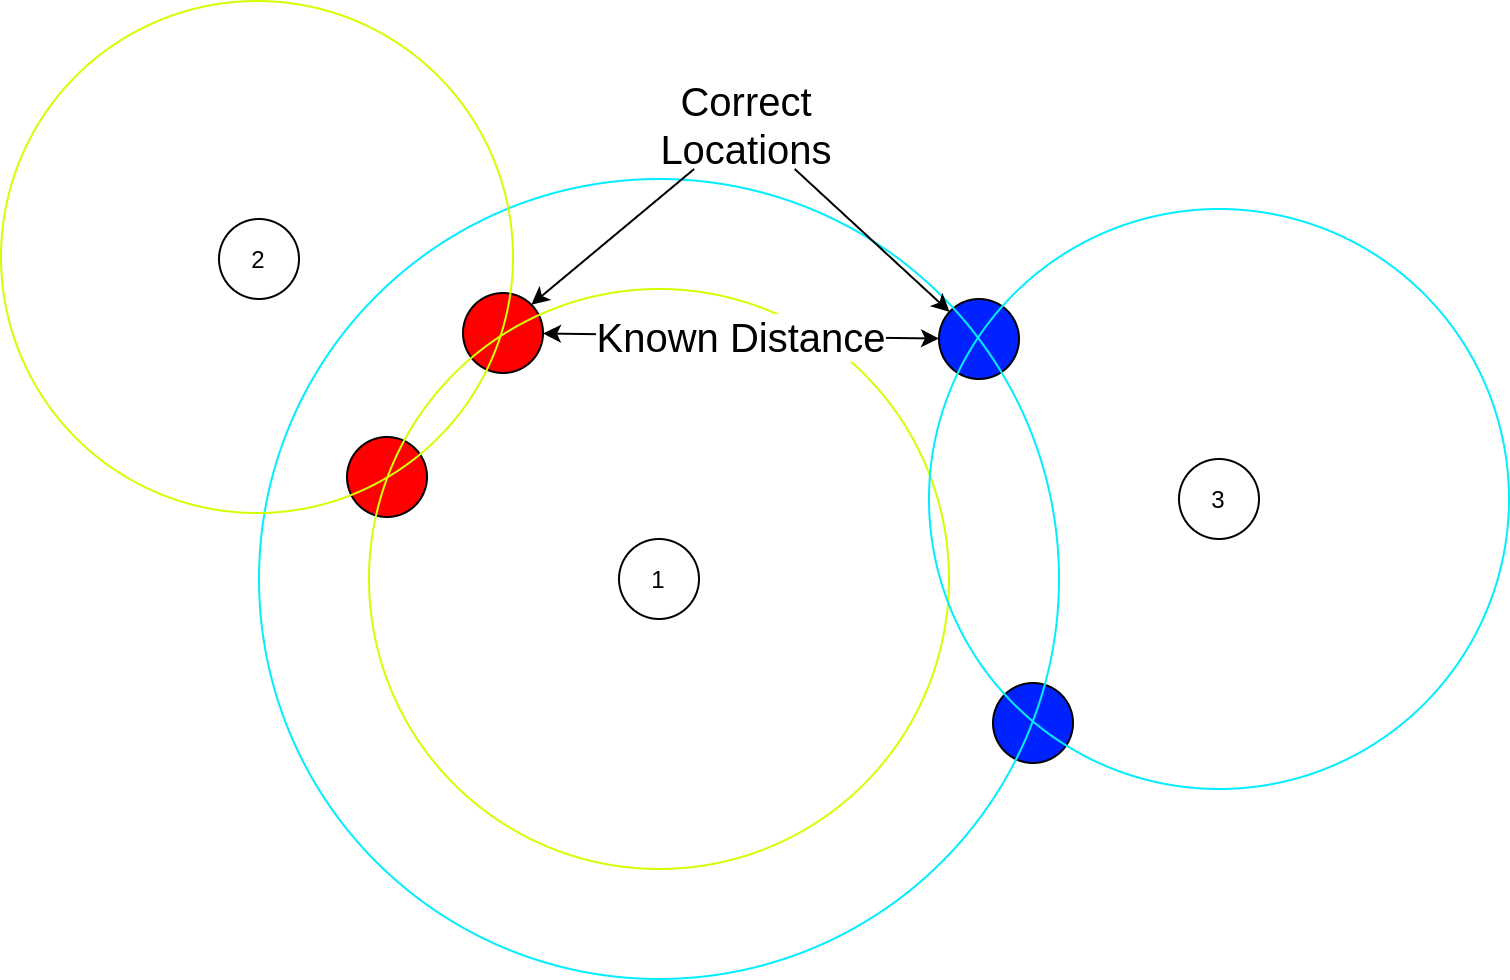
\includegraphics[width=0.8\textwidth]{images/unknown_point_finding.png}
	\caption{Finding a location of points without partial information}
	\label{fig:partial_point_find}
\end{figure}

 